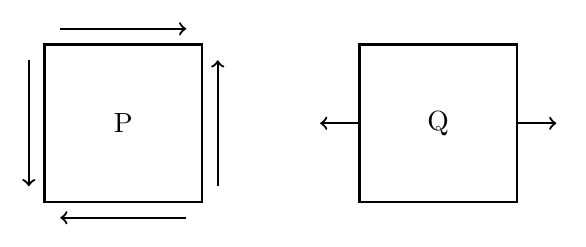
\begin{tikzpicture}

% Square P
\draw[thick] (0, 0) rectangle (2, 2);
\node at (1, 1) {P};

% Arrows around P
\draw[->, thick] (0.2, 2.2) -- (1.8, 2.2);
\draw[->, thick] (2.2, 0.2) -- (2.2, 1.8);
\draw[->, thick] (-0.2, 1.8) -- (-0.2, 0.2);
\draw[->, thick] (1.8, -0.2) -- (0.2, -0.2);

% Square Q
\draw[thick] (4, 0) rectangle (6, 2);
\node at (5, 1) {Q};

% Arrows around Q
\draw[<-, thick] (3.5, 1) -- (4, 1);
\draw[->, thick] (6, 1) -- (6.5, 1);

\end{tikzpicture}
